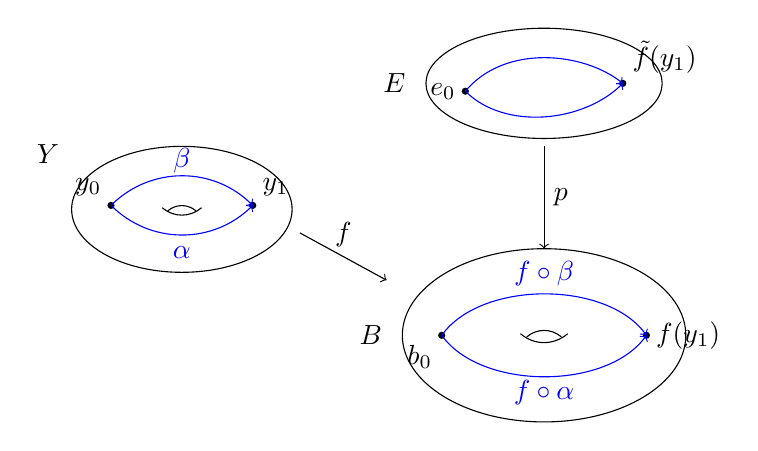
\begin{tikzpicture}
% Y
\draw (0,0) ellipse (1.4 and 0.8);
\node at (-1.7,0.7) {$Y$};
\draw (-0.25,0.02) to[bend right=40] (0.25,0.02);
\draw (-0.18,-0.02) to[bend left=40] (0.18,-0.02);
\fill (-0.9,0.05) circle (1.3pt) node[above left] {$y_0$};
\fill (0.9,0.05) circle (1.3pt) node[above right] {$y_1$};
\draw[blue, ->] (-0.9,0.05) .. controls (-0.4,0.55) and (0.4,0.55) .. (0.9,0.05);
\draw[blue, ->] (-0.9,0.05) .. controls (-0.4,-0.45) and (0.4,-0.45) .. (0.9,0.05);
\node[blue] at (0,0.62) {$\beta$};
\node[blue] at (0,-0.55) {$\alpha$};
% B
\draw (4.6,-1.6) ellipse (1.8 and 1.1);
\node at (2.4,-1.6) {$B$};
\draw (4.3,-1.58) to[bend right=40] (4.9,-1.58);
\draw (4.38,-1.62) to[bend left=40] (4.82,-1.62);
\fill (3.3,-1.6) circle (1.3pt) node[below left] {$b_0$};
\fill (5.9,-1.6) circle (1.3pt) node[right] {$f(y_1)$};
\draw[blue, ->] (3.3,-1.6) .. controls (3.8,-0.9) and (5.4,-0.9) .. (5.9,-1.6);
\draw[blue, ->] (3.3,-1.6) .. controls (3.8,-2.3) and (5.4,-2.3) .. (5.9,-1.6);
\node[blue] at (4.6,-0.82) {$f\circ\beta$};
\node[blue] at (4.6,-2.33) {$f\circ\alpha$};
% E
\draw (4.6,1.6) ellipse (1.5 and 0.7);
\node at (2.7,1.6) {$E$};
\fill (3.6,1.5) circle (1.3pt) node[left] {$e_0$};
\fill (5.6,1.6) circle (1.3pt) node[above right] {$\tilde f(y_1)$};
\draw[blue, ->] (3.6,1.5) .. controls (4.1,2.1) and (5.1,2.0) .. (5.6,1.6);
\draw[blue, ->] (3.6,1.5) .. controls (4.1,1.0) and (5.1,1.1) .. (5.6,1.6);
% maps
\draw[->] (1.5,-0.3) -- node[above] {$f$} (2.6,-0.9);
\draw[->] (4.6,0.8) -- node[right] {$p$} (4.6,-0.5);
\end{tikzpicture}
